
        \documentclass[spanish, 11pt]{exam}

        %These tell TeX which packages to use.
        \usepackage{array,epsfig}
        \usepackage{amsmath, textcomp}
        \usepackage{amsfonts}
        \usepackage{amssymb}
        \usepackage{amsxtra}
        \usepackage{amsthm}
        \usepackage{mathrsfs}
        \usepackage{color}
        \usepackage{multicol, xparse}
        \usepackage{verbatim}


        \usepackage[utf8]{inputenc}
        \usepackage[spanish]{babel}
        \usepackage{eurosym}

        \usepackage{graphicx}
        \graphicspath{{../img/}}



        \printanswers
        \nopointsinmargin
        \pointformat{}

        %Pagination stuff.
        %\setlength{\topmargin}{-.3 in}
        %\setlength{\oddsidemargin}{0in}
        %\setlength{\evensidemargin}{0in}
        %\setlength{\textheight}{9.in}
        %\setlength{\textwidth}{6.5in}
        %\pagestyle{empty}

        \let\multicolmulticols\multicols
        \let\endmulticolmulticols\endmulticols
        \RenewDocumentEnvironment{multicols}{mO{}}
         {%
          \ifnum#1=1
            #2%
          \else % More than 1 column
            \multicolmulticols{#1}[#2]
          \fi
         }
         {%
          \ifnum#1=1
          \else % More than 1 column
            \endmulticolmulticols
          \fi
         }
        \renewcommand{\solutiontitle}{\noindent\textbf{Sol:}\enspace}

        \newcommand{\samedir}{\mathbin{\!/\mkern-5mu/\!}}

        \newcommand{\class}{1º Bachillerato}
        \newcommand{\examdate}{\today}

        \newcommand{\tipo}{A}


        \newcommand{\timelimit}{50 minutos}



        \pagestyle{head}
        \firstpageheader{
\includegraphics[width=0.2\columnwidth]{header_left}}{\textbf{Departamento de Matemáticas\linebreak \class}\linebreak \examnum}{
\includegraphics[width=0.1\columnwidth]{header_right}}
        \runningheader{\class}{\examnum}{Página \thepage\ of \numpages}
        \runningheadrule

        \newcommand{\examnum}{41 - Estadística Unidimensional}
        \begin{document}
        \begin{questions}
        \question p089e01 - Las calificaciones de un grupo de alumnos han sido: 9 6 5 0 1 5 7 9 10 7 5 1 2 5 7 6 3 4 6 8 8 6 4 4 6 5 3 5 7 7 8 7 2 2
        \begin{multicols}{1} 
        \begin{parts} \part[1] Realiza una tabla de frecuencias  \begin{solution}   \begin{tabular}{rrrrrrr}
\hline
   x\_i &   f\_i &   F\_i &       r\_i &       R\_i &      \%\_i &      \%A\_i \\
\hline
     0 &     1 &     1 & 0.0294118 & 0.0294118 &  2.94118 &   2.94118 \\
     1 &     2 &     3 & 0.0588235 & 0.0882353 &  5.88235 &   8.82353 \\
     2 &     3 &     6 & 0.0882353 & 0.176471  &  8.82353 &  17.6471  \\
     3 &     2 &     8 & 0.0588235 & 0.235294  &  5.88235 &  23.5294  \\
     4 &     3 &    11 & 0.0882353 & 0.323529  &  8.82353 &  32.3529  \\
     5 &     6 &    17 & 0.176471  & 0.5       & 17.6471  &  50       \\
     6 &     5 &    22 & 0.147059  & 0.647059  & 14.7059  &  64.7059  \\
     7 &     6 &    28 & 0.176471  & 0.823529  & 17.6471  &  82.3529  \\
     8 &     3 &    31 & 0.0882353 & 0.911765  &  8.82353 &  91.1765  \\
     9 &     2 &    33 & 0.0588235 & 0.970588  &  5.88235 &  97.0588  \\
    10 &     1 &    34 & 0.0294118 & 1         &  2.94118 & 100       \\
\hline
\end{tabular}   \end{solution} \part[1] Realiza un diagrama de barras y un polígono de frecuencias  \begin{solution}   \\ 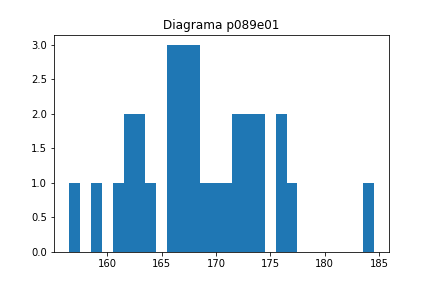
\includegraphics[width=1\columnwidth]{p089e01}   \end{solution} \part[1] Calcular los parámetros de centralización  \begin{solution}   {'media': 5.294117647058823, 'mediana': 5.5, 'moda': ModeResult(mode=array([5]), count=array([6]))}   \end{solution} \part[1] Calcular los parámetros de posición  \begin{solution}   {'Q1': 4.0, 'Q3': 7.0}   \end{solution} \part[1] Calcular los parámetros de dispersión  \begin{solution}   {'rango': 10, 'varianza': 6.031141868512111, 'desviación típica': 2.45583832295860, 'coeficiente variación': 0.463880572114402}   \end{solution}
        \end{parts}
        \end{multicols}
        \question p089e02 - Estos datos reflejan el tiempo, en minutos, que tardan en llegar a su centro escolar varios alumnos. 10 15 11 11 14 14 11 14 17 11 17 15 10 16 12 12 13 16 13 16 18 12 18 16
        \begin{multicols}{1} 
        \begin{parts} \part[1] Realiza una tabla de frecuencias  \begin{solution}   \begin{tabular}{rrrrrrr}
\hline
   x\_i &   f\_i &   F\_i &       r\_i &       R\_i &      \%\_i &      \%A\_i \\
\hline
    10 &     2 &     2 & 0.0833333 & 0.0833333 &  8.33333 &   8.33333 \\
    11 &     4 &     6 & 0.166667  & 0.25      & 16.6667  &  25       \\
    12 &     3 &     9 & 0.125     & 0.375     & 12.5     &  37.5     \\
    13 &     2 &    11 & 0.0833333 & 0.458333  &  8.33333 &  45.8333  \\
    14 &     3 &    14 & 0.125     & 0.583333  & 12.5     &  58.3333  \\
    15 &     2 &    16 & 0.0833333 & 0.666667  &  8.33333 &  66.6667  \\
    16 &     4 &    20 & 0.166667  & 0.833333  & 16.6667  &  83.3333  \\
    17 &     2 &    22 & 0.0833333 & 0.916667  &  8.33333 &  91.6667  \\
    18 &     2 &    24 & 0.0833333 & 1         &  8.33333 & 100       \\
\hline
\end{tabular}   \end{solution} \part[1] Realiza un diagrama de barras y un polígono de frecuencias  \begin{solution}   \\ 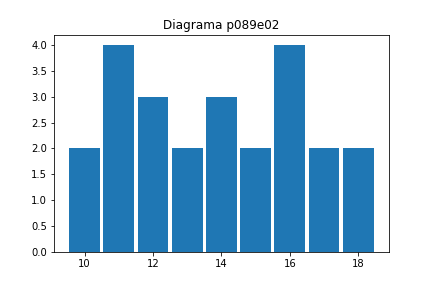
\includegraphics[width=1\columnwidth]{p089e02}   \end{solution} \part[1] Calcular los parámetros de centralización  \begin{solution}   {'media': 13.833333333333334, 'mediana': 14.0, 'moda': ModeResult(mode=array([11]), count=array([4]))}   \end{solution} \part[1] Calcular los parámetros de posición  \begin{solution}   {'Q1': 11.75, 'Q3': 16.0}   \end{solution} \part[1] Calcular los parámetros de dispersión  \begin{solution}   {'rango': 8, 'varianza': 6.222222222222221, 'desviación típica': 2.49443825784929, 'coeficiente variación': 0.180320837916816}   \end{solution}
        \end{parts}
        \end{multicols}
        
    \end{questions}
    \end{document}
    